%%%%% Preamble %%%%%%%
\documentclass[aps,prd,twocolumn,floatfix,showpacs,superscriptaddress,nofootinbib]{revtex4-1}
\pdfoutput=1
\usepackage{epsfig, subfigure}
\usepackage{setspace}
\usepackage{booktabs, tabularx} 
\usepackage{amsmath,bm,bbm}
\usepackage{hyperref}
\usepackage{graphicx}
\usepackage{enumerate}
\usepackage{dcolumn}% Align table columns on decimal point
\usepackage{bm}% bold math
\usepackage{longtable}

\usepackage{color}



%%%%% Literary Shortcuts %%%%%%%%%
\newcommand{\ie}{{\it i.e. }}
\newcommand{\eg}{{\it e.g. }}
\newcommand{\etal}{{\it et al. }}


\mathchardef\mhyphen="2D

\hyphenpenalty=10000
\tolerance=100
\widowpenalty=10000
\clubpenalty=10000

\begin{document}

\title{Whatever}

\author{Xiao Fang}
\affiliation{Department of Physics, Ohio State University, 191 W.~Woodruff Ave., Columbus, OH~~43210, USA}

\date{\today}


\maketitle

int main\{\\
\}

\bibliographystyle{ieeetr}
\bibliography{mybib}

\newpage

\appendix
\section{Lensing Magnetic Field Contamination}
In this Appendix, we first briefly derive the power spectra of the transverse shear components of weak lensing. Then we estimate the magnetic field contamination due to lensing. At the end, we consider CMB lensing as an additional source of information to help diminish the contamination.

\subsection{Transverse Shear Power Spectrum}
The formalism for the two-dimensional weak lensing carried out, for example, in \cite{Weinberg201387} is quite straightforward to be generalized to 3-dimensional case, where lensing maps the intrinsic image of sources on the sky, namely the source space, onto the observed sky, namely the image space. Any position on the sky can be denoted by its angular coordinates $(\theta_1,\theta_2)$ and its comoving distance $D$ or its redshift $z$.

Analogous to 2-dimensional weak lensing, we have
\begin{equation}
\theta_i^S=\theta_i+\frac{\partial\psi}{\partial\theta_i},\ i=1,2,3,
\label{lensingmapping}
\end{equation}
representing  that sources intrinsicly at position $(\theta_1^S,\theta_2^S,\theta_3^S)$ are related to the apparent position $(\theta_1,\theta_2,\theta_3)$ by the lensing potential $\psi$. Note that we assume the universe is flat, so that the angular coordinate components satisfy
\begin{equation}
\theta_i=\frac{\Delta x_i}{D},\ i=1,2,3,
\end{equation}
where $\Delta x_{1,2}$ is the comoving coordinates on the image plane near the source. The third coordinate $\Delta x_3$ is a small comoving deviation from the origin (which can be chosen arbitarily in the image space near the source) along the line of sight, so that it is related to redshift by $\Delta x_3=\Delta z/H$.

By taking the derivative of Eqn.(\ref{lensingmapping}), we find the Jacobian of the coordinate transformation from the image space to the source space,
\begin{equation}
\frac{\partial\theta_i^S}{\partial\theta_j}=\delta_{ij}+\frac{\partial^2\psi}{\partial\theta_i\partial\theta_j}=(1+\kappa)I_{ij}+\gamma_{ij},\ \ \ i,j=1,2,3,
\label{lensingtsf}
\end{equation}
where we decompose the symmetric $\partial^2\psi/\partial\theta_i\partial\theta_j$ as the sum of a diagonal matrix and a symmetric traceless matrix $\bm{\gamma}$. They represent the effect of magnification and shear, respectively. There are 5 independent shear components.

Now we switch to the 2-dimentional Fourier space, \ie from $\hat{n}\equiv(\theta_1,\theta_2)$ to $\vec{l}\equiv(l_1,l_2)$, where we put a tilde above the quantities. The $\tilde{\gamma}_{13},\tilde{\gamma}_{23}$ components are the transverse shear components that we care about. Let's calculate the power spectrum of $\gamma_{13}$ first.

The 2D Fourier transform of the lensing potential is
\begin{equation}
\tilde{\psi}(\vec{l},D)=\int_\Omega\psi(D,\hat{n})e^{-i\vec{l}\cdot\hat{n}}\ d\theta_1 d\theta_2.
\label{potentialFourier}
\end{equation}
Note that the lensing potential $\psi$ is given by
\begin{equation}
\psi(D,\hat{n})=
-2\int_0^{D}[\cot_K(D_1)-\cot_K(D)]\Phi(D_1,\hat{n})dD_1,
\label{lensingpotential}
\end{equation}
where $\Phi$ is the Newtonian gravitational potential and the cotangentlike function is hyperbolic for flat universe, \ie $\cot_K(D)=1/D$. One can show that
\begin{equation}
\frac{\partial\tilde{\psi}(\vec{l},z)}{\partial\theta_3}=-\frac{2}{D}\int_0^D dD_1\tilde{\Phi}(D_1,\vec{l}),
\end{equation}
where $\tilde{\Phi}$ is the 2D Fourier transform of $\Phi$. Now we obtain
\begin{align}
&\langle\tilde{\gamma}_{13}^*(\vec{l},z)\tilde{\gamma}_{13}(\vec{l}',z')\rangle=\left\langle l_1l_1'\frac{\tilde{\psi}^*(\vec{l},z)}{\partial\theta_3}\frac{\tilde{\psi}(\vec{l}',z')}{\partial\theta_3}\right\rangle\nonumber\\
&=\frac{4l_1l_1'}{D(z)D(z')}\int_0^{D(z)}dD_1\int_0^{D(z')}dD_1'\langle\tilde{\Phi}^*(D_1,\vec{l})\tilde{\Phi}(D_1',\vec{l}')\rangle.
\end{align}
Define
\begin{equation}
\tilde{\Phi}(D_1,\vec{l})\equiv\int_{-\infty}^{\infty}\tilde{\tilde{\Phi}}(l_3,\vec{l})e^{il_3D_1}\frac{dl_3}{2\pi},
\end{equation}
we can write
\begin{align}
\langle\tilde{\Phi}^*(D_1,\vec{l})\tilde{\Phi}(D_1',\vec{l}')\rangle=\int\int&\frac{dl_3}{2\pi}\frac{dl_3'}{2\pi}\langle\tilde{\tilde{\Phi}}^*(l_3,\vec{l})\tilde{\tilde{\Phi}}(l_3',\vec{l}')\rangle\nonumber\\
&\times e^{i(l_3'D_1'-l_3D_1)}. \label{eq:doubletilde}
\end{align}
Here $\tilde{\tilde{\Phi}}$ is actually the 3D Fourier transform of $\Phi$, so we can assume that different modes are uncorrelated, which implies
\begin{equation}
\langle\tilde{\tilde{\Phi}}^*(l_3,\vec{l})\tilde{\tilde{\Phi}}(l_3',\vec{l}')\rangle=(2\pi)^3\delta(l_3-l_3')\delta^2(\vec{l}-\vec{l}')P_{\Phi}(\sqrt{l_3^2+\vert\vec{l}\vert^2}).
\end{equation}
Substituting into Eqn.(\ref{eq:doubletilde}) and applying the Limber's approximation: $l_3\ll\vert\vec{l}\vert$, we obtain
\begin{equation}
\langle\tilde{\Phi}^*(D_1,\vec{l})\tilde{\Phi}(D_1',\vec{l}')\rangle\simeq(2\pi)^2\delta^2(\vec{l}-\vec{l}')P_{\Phi}(\vert\vec{l}\vert)\delta(D_1'-D_1).
\end{equation}
Thus, for $z\leq z'$ we have
\begin{align}
&\langle\tilde{\gamma}_{13}^*(\vec{l},z)\tilde{\gamma}_{13}(\vec{l}',z')\rangle\nonumber\\
&=\frac{4}{D(z)D(z')}l_1l_1'(2\pi)^2\delta^2(\vec{l}-\vec{l}')\int_0^{D(z)}dD_1P_{\Phi}(l),
\end{align}
where $l\equiv\vert\vec{l}\vert$ and $P_{\Phi}(l)$ is the angular power spectrum,
\begin{equation}
P_{\Phi}(l)=\frac{P_{\Phi}(k=l/D_1)}{D_1^2}=\left[\frac{3}{2}\Omega_mH_0^2(1+z_1)\right]^2\frac{P_{\delta}(k,z_1)}{k^4D_1^2},
\end{equation}
where $P_\delta$ is the matter power spectrum.

If we define the power spectrum $P_{13}(\vec{l},z,z')$ of $\gamma_{13}$ components as
\begin{equation}
\langle\tilde{\gamma}_{13}^*(\vec{l},z)\tilde{\gamma}_{13}(\vec{l}',z')\rangle\equiv(2\pi)^2P_{13}(\vec{l},z,z')\delta^2(\vec{l}-\vec{l}'),
\end{equation}
then we have
\begin{equation}
P_{13}(\vec{l},z,z')=\frac{4l_1^2}{D(z)D(z')}\int_0^{D(z)}dD_1P_{\Phi}(l).
\end{equation}

There are similar results for the power spectrum $P_{23}$ of $\gamma_{23}$ component. Furthermore, we can define the transverse power spectrum $P_t$ as follows,
\begin{align}
P_t(l,z,z')\equiv &P_{13}+P_{23}\nonumber\\
=&\frac{4l^2}{D(z)D(z')}\int_0^{D(z)}dD_1P_{\Phi}(l).
\end{align}
This transverse power spectrum does not depend on the components but the magnitude of the angular wave number vector.

\begin{figure}
\centering
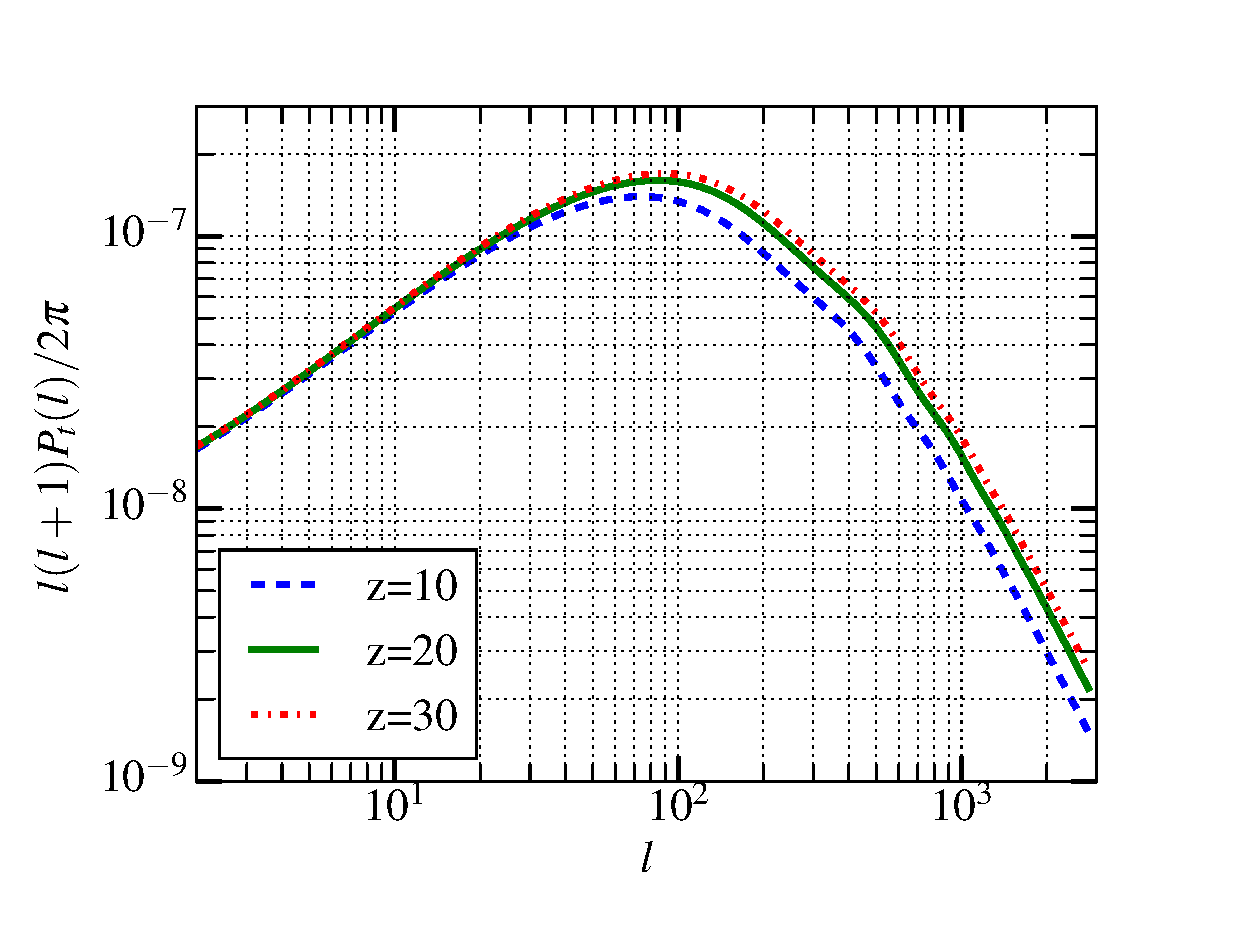
\includegraphics[scale=0.45]{pt_2.eps}
\caption{The transverse power spectra for sources at redshifts $z=10$(bottom), $20$ and $30$(top), predicted for the WMAP 7-year best fit cosmology ($\Omega_m=0.265,\sigma_8=0.8,H_0=71.9\ \mathrm{km\ s^{-1}Mpc^{-1}}$).}
\label{Pt}
\end{figure}

If the separation between $z$ and $z'$ are negligible, i.e. $z=z'$, we have
\begin{equation}
P_t(l,z)=\frac{4l^2}{D^2(z)}\int_0^{D(z)}dD_1P_{\Phi}(l).
\end{equation}
The results are shown in Fig.\ref{Pt}.

\subsection{Lensing Contamination}
Venumadhav \etal\cite{Venumadhav:2014tqa} has found the expression of the brightness temperature fluctuation $\delta T_b$ as a function of the magnitude of magnetic fields, \ie Eqn.(1){\color{red} (Need to refer to the equation in your paper)}. To make the derivation concise, we define several quantities as below.
\begin{align}
\bar{x}_{\rm B}&\equiv\frac{x_{\rm B}}{B} = \frac{g_{\rm e} \mu_{\rm B} T_*}{2 \hbar A T_\gamma},\\
A&\equiv\left( 1 - \frac{T_\gamma}{T_{\rm s}} \right) x_{1{\rm s}} \left( \frac{1+z}{10} \right)^{1/2},\\
C&\equiv0.128 \ {\rm mK} \left( \frac{T_\gamma}{T_{\rm s}} \right) x_{1{\rm s}} \left( \frac{1+z}{10} \right)^{1/2},\\
\mu&\equiv\frac{C}{10}\frac{x_B}{(1+x_{\alpha,(2)}+x_{c,(2)})^2},\\
\lambda&\equiv 13.2-C-\frac{C}{20}\frac{1}{1+x_{\alpha,(2)}+x_{c,(2)}},\\
q&\equiv 39.6-3C-\frac{C}{60}\frac{1}{1+x_{\alpha,(2)}+x_{c,(2)}}.
\end{align}


The power spectrum of the brightness temperature is related to the matter power spectrum $P_\delta(k)$ by
\begin{equation}
P_{T_b}(\bm k)=\left\vert\frac{\partial\delta T_b}{\partial\delta}\right\vert^2 P_\delta(k).
\end{equation}
The transfer function $\partial\delta T_b/\partial\delta$ is given by taking derivative of (1){\color{red} (Need to refer to the equation in your paper)}, \ie
\begin{eqnarray}
\frac{\partial\delta T_b}{\partial\delta}&&=A\left[(26.4-2C)\left(1 + (\hat{\bm k} \cdot \hat{\bm n})^2\right)\right. \nonumber\\
&&\left.-\frac{C}{15}\sum_m \frac{4\pi}{5}\frac{Y_{2m}(\hat{\bm k})[Y_{2m}(\hat{\bm n})]^*}{1+x_{\alpha,(2)}+x_{c,(2)}-imx_B}\right],
\label{eq:bttsf}
\end{eqnarray}

By expanding Eqn.(\ref{eq:bttsf}) for small magnetic field $B$ (\ie small $x_B$), we will obtain a precession correction on the original $P_{T_b}$ profile. The tangent of the precession angle $\theta_{pr}$ is proportional to the magnitude of the magnetic field applied.

To see that, let's first define our coordinate system as shown in Fig.\ref{fig:coordinate}. The unit vectors then will be $\hat{k}=(\pi/2,\varphi)$ and $\hat{n}=(\pi/2,0)$, where the first coordinate represents the angle between the Direction \#2 and the vector. The expansion becomes
\begin{equation}
\frac{\partial\delta T_b}{\partial\delta}=A(q+\lambda\cos 2\varphi+\mu\sin 2\varphi).
\label{eq:Tbtsf_simplified}
\end{equation}
\begin{figure}
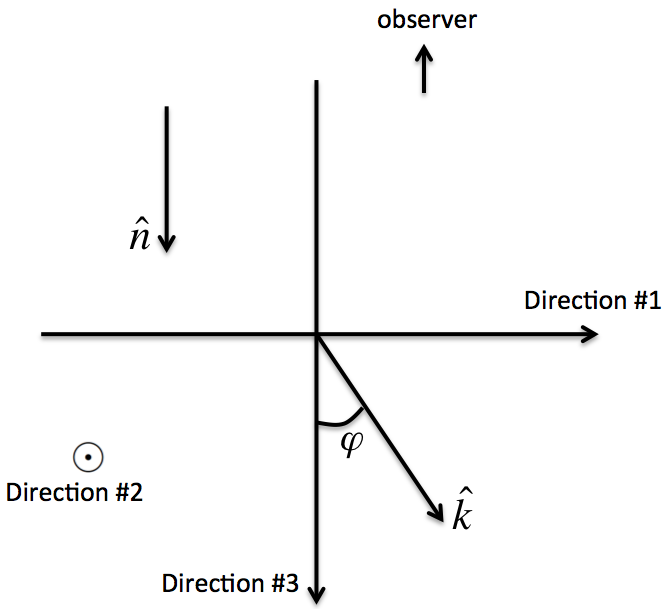
\includegraphics[scale=0.3]{coordinate.png}
\caption{The coordinate system}
\label{fig:coordinate}
\end{figure}

Due to the $\sin 2\varphi$ term contributed by the small magnetic field, the original profile gets a small precession angle $\theta_{pr}$
\begin{equation}
\theta_{pr}\simeq\tan\theta_{pr}=-\frac{\mu}{\lambda},
\end{equation}

Thus, if we measure the precession angle $\theta_{pr}$ in the power spectra of $T_b$, we can determine the magnitude of the magnetic field.

Next we will show that the transverse components of the weak lensing can also produce a similar precession angle.

In the 3D Cartesian coordinate, the unit vectors are written as
\begin{equation}
\hat{k}=(\sin\varphi,0,\cos\varphi),\ \hat{n}=(0,0,1),
\end{equation}
and they are distorted into
\begin{align}
\hat{k}'&=\left(\begin{array}{c}
(1+\kappa+\gamma_{11})\sin\varphi+\gamma_{13}\cos\varphi\\
\gamma_{12}\sin\varphi+\gamma_{23}\cos\varphi\\
\gamma_{13}\sin\varphi+(1+\kappa+\gamma_{33})\cos\varphi
\end{array}\right),\nonumber\\
\hat{n}'&=(\gamma_{13},\gamma_{23},1+\kappa+\gamma_{33}).
\end{align}
Since the shearing components are all very small, by taking the first order, we obtain the shear only change $\varphi$ by
\begin{equation}
\Delta\varphi\simeq\sin\Delta\varphi\simeq-2\gamma_{13}.
\end{equation}
Thus, if we don't have magnetic field (\ie $x_B=0$), due to the weak lensing, the transfer function (\ref{eq:Tbtsf_simplified}) will become
\begin{equation}
\frac{\partial\delta T_b}{\partial\delta}=A[q+\lambda(\cos 2\varphi+4\gamma_{13}\sin 2\varphi)].
\label{eq:Tbtsf_shear}
\end{equation}
Since the weak lensing also spurs the $k$ in $P_\delta(k)$, we need to find the relation between $P_\delta(k')$ and $P_\delta(k)$. To the first order, we can find
\begin{equation}
k'=k(1+\kappa+\gamma_{11}\sin^2\varphi+\gamma_{33}\cos^2\varphi+2\gamma_{13}\sin\varphi\cos\varphi).
\end{equation}
Since $P_\delta(k)\propto k^{n_{\rm eff}}$, we have
\begin{align}
P_{T_b}(\vec{k}')=&\left\vert\frac{\partial\delta T_b}{\partial\delta}[1+\kappa+\gamma_{11}\sin^2\varphi+\gamma_{33}\cos^2\varphi\right.\nonumber\\
&\left.+2\gamma_{13}\sin\varphi\cos\varphi]^{n_{\rm eff}/2}]\right\vert^2P_\delta(k),
\end{align}
where $n_{\rm eff}$ is the effective spectral index. We can see all the quadropole features in the power spectra of $T_b$ come from the modified transfer function.

After expanding, keeping the first-order terms and neglecting small octupole terms, we can obtain the modified transfer function, and find the precession angle again, given by the negative ratio of the two coefficients of the quadrupole terms,
\begin{equation}
\theta_{pr}'\simeq-\left(4+\frac{n_{\rm eff}}{2}\frac{q}{\lambda}\right)\gamma_{13}.
\end{equation}
This precession angle is made by the transverse weak lensing component instead of the magnetic field, but the effect it makes looks like there is a (fake) magnetic field such that
\begin{equation}
\frac{\mu}{\lambda}=\left(4+\frac{n_{\rm eff}}{2}\frac{q}{\lambda}\right)\gamma_{13},
\end{equation}
where we can solve for the (fake) comoving magnetic field
\begin{align}
B_{\rm lensing,13}&=\frac{10(1+x_{\alpha,(2)}+x_{c,(2)})^2(4\lambda+\frac{n_{\rm eff}}{2}q)}{C\bar{x}_{\rm B}(1+z)^2}\gamma_{13}\nonumber\\
&\equiv\alpha\gamma_{13}.
\end{align}
Finally, we find the power spectrum of the comoving lensing magnetic field
\begin{equation}
P_B^{\rm lensing,13}(l)=\left\vert\frac{\partial B_{\rm lensing,13}}{\partial\gamma_{13}}\right\vert^2 P_{\gamma_{13}}(l)=\alpha^2 P_{\gamma_{13}}(l).
\end{equation}
Note that this power spectrum is only the contribution from $\gamma_{13}$ component because we assume $\hat{k}$ to sit on the "1-3" plane. For any position on the sky, one has the choice to rotate his coordinate system to maximize or minimize $P_{\gamma_{13}}$. However, randomly, the total power spectrum of comoving lensing magnetic field picks up an average value, \ie the half maximum,
\begin{equation}
P_B^{\rm lensing}(l)=\frac{\alpha^2}{2} P_t(l),
\end{equation}
\begin{equation}
\Delta_{B}^{\rm lensing}(l)=\sqrt{\frac{l(l+1)}{2\pi}P_B^{\rm lensing}(l)}
\end{equation}

For a survey with $\Omega_{\rm survey}=1{\rm sr}$, the scale of interest is about $l=6$. The scale of matter fluctuations relavant to the observed signals is determined by the resolution of the inferometers as
\begin{equation}
k\sim \frac{2\pi L}{\lambda_0(1+z)D}\sim 1,
\end{equation}
corresponding to $n_{\rm eff}\sim -2.274$.

\subsection{De-lensing}
Here is the basic idea of de-lensing.

Consider we have a signal $\vec{x}$, expressed by random variables $x_1,x_2,\cdots,x_M$, so that when we measure the values of $x_1,x_2,\cdots,x_M$, we get variances $C_{11},C_{22},\cdots,C_{MM}$, as well as their covariances. Suppose we can detect another signal $\vec{y}$, expressed by random variables $y_1,y_2,\cdots,y_N$, with their variances and covariances, we can use them to further constrain the variances of measuring $\vec{x}$, if $\vec{x}$ and $\vec{y}$ are correlated.

In the simplest case, we assume $\vec{x}$, $\vec{y}$  are Gaussian random variables and $\vec{x},\vec{y}$ obey the 2-dimensional Gaussian distribution. Then we can write the covariance matrix as
\begin{equation}
\mathbf{C}=\left(\begin{array}{cc}
\mathbf{C}^{xx} & \mathbf{C}^{xy}\\
\mathbf{C}^{yx} & \mathbf{C}^{yy}
\end{array}\right),
\end{equation}
where $\mathbf{C}$ is a $(M+N)\times(M+N)$ matrix.

Now we can work out the probability of obtaining $\vec{x}$ given $\vec{y}$:
\begin{widetext}
\begin{align}
P(\vec{x}\vert\vec{y})&=\frac{P(\vec{x},\vec{y})}{P(\vec{y})}\nonumber\\
&=(2\pi)^{-M/2}(\det\mathbf{C}_{post}^{xx})^{-1/2}\exp\left\lbrace -\frac{1}{2}\left[\vec{x}+\left(\left(\mathbf{C}^{-1}\right)^{xx}\right)^{-1}\left(\mathbf{C}^{-1}\right)^{xy}\vec{y}\right]^T\left(\mathbf{C}_{post}^{xx}\right)^{-1}\left[\vec{x}+\left(\left(\mathbf{C}^{-1}\right)^{xx}\right)^{-1}\left(\mathbf{C}^{-1}\right)^{xy}\vec{y}\right]\right\rbrace.
\label{eq:posterior}
\end{align}
\end{widetext}

The last line shows that the posterior probability of obtaining signal $\vec{x}$ still satisfies a Gaussian distribution, with shifted mean values of $\vec{x}$ and a posterior covariance matrix $\mathbf{C}_{post}^{xx}$:
\begin{align}
\det\mathbf{C}_{post}^{xx}&\equiv\frac{\det\mathbf{C}}{\det\mathbf{C}^{yy}},\nonumber\\
\langle\vec{x}\rangle\vert_{\vec{y}}&\equiv -\left(\left(\mathbf{C}^{-1}\right)^{xx}\right)^{-1}\left(\mathbf{C}^{-1}\right)^{xy}\vec{y},\nonumber\\
\left(\mathbf{C}_{post}^{xx}\right)^{-1}&=\left(\mathbf{C}^{-1}\right)^{xx}.
\end{align}

Finally we have this relation:
\begin{equation}
\mathbf{C}_{post}^{xx}=\left[\left(\mathbf{C}^{-1}\right)^{xx}\right]^{-1}.
\end{equation}

We can further apply the blockwise inversion formula to prove that by doing this, we can get a better constraint on $\vec{x}$, \ie lower the variance in $\mathbf{C}^{xx}$.

Now applying to the de-lensing case, $\gamma_{13}$ is the signal we want to constrain, and CMB convergence $\kappa$ is the additional signal provided. Going through a very similar derivation, we obtain the power spectrum of CMB convergence, as well as the cross spectra between transverse shear components and CMB convergence,
\begin{align}
P_{\kappa}(\vec{l})&=l^4\int_0^{D_0}dD_1\left(\frac{1}{D_1(z_1)}-\frac{1}{D_0}\right)^2P_\Phi(l),\nonumber\\
P_{13,\kappa}(\vec{l},z_i)&=\frac{2il_1l^2}{D(z_i)}\int_0^{D(z_i)}dD_1\left(\frac{1}{D_1(z_1)}-\frac{1}{D_0}\right)P_\Phi(l),
\end{align}
where $D_0$ is the comoving distance of the CMB.

For the $N$ redshift slices and the angular scale $l$ that we are interested in, we can write the covariance matrix as a $(N+1)\times(N+1)$ matrix,
\begin{equation}
\mathbf{C}_l=\left(\begin{array}{ll}
\mathbf{P}^{13} & \mathbf{P}^{13,\kappa}\\
\mathbf{P}^{\kappa,13} & \mathbf{P}^{\kappa}
\end{array}\right),
\end{equation}
where $\mathbf{P}^{13}$ is the $N\times N$ matrix formed by $P_{13}(\vec{l},z_i,z_j)$, $\mathbf{P}^{13,\kappa}$ the $N\times 1$ matrix formed by $P_{13,\kappa}(\vec{l},z_i)$, $\mathbf{P}^{\kappa}$ the number $P_{\kappa}(\vec{l})$. $\mathbf{P}^{\kappa,13}$ can be obtained by taking Hermitian conjugate of $\mathbf{P}^{13,\kappa}$.

After de-lensing, the posterior convariance matrix of $\mathbf{P}^{13}$ becomes
\begin{equation}
\mathbf{P}_{\rm post}^{13}=\left( (\mathbf{C}_l^{-1})^{NN} \right)^{-1},
\end{equation}
where $(\cdots)^{NN}$ means taking the upper left $N\times N$ submatrix. Note that this time we need to do the average over the choices of coordinate for the posterior power spectra instead of the prior ones. That means we set $l_1=l$ at first, after calculating the posteriors, we average them over the choices of coordinate, which turns out to just introduce a factor of $1/2$ as previous.

The result is shown in Figure.\ref{fig:ps_B}. The de-lensing procedure slightly decreases the transverse shear power spectra, hence reducing the their contamination on the stochastic magnetic field signals.

\begin{figure}[h]
\centering
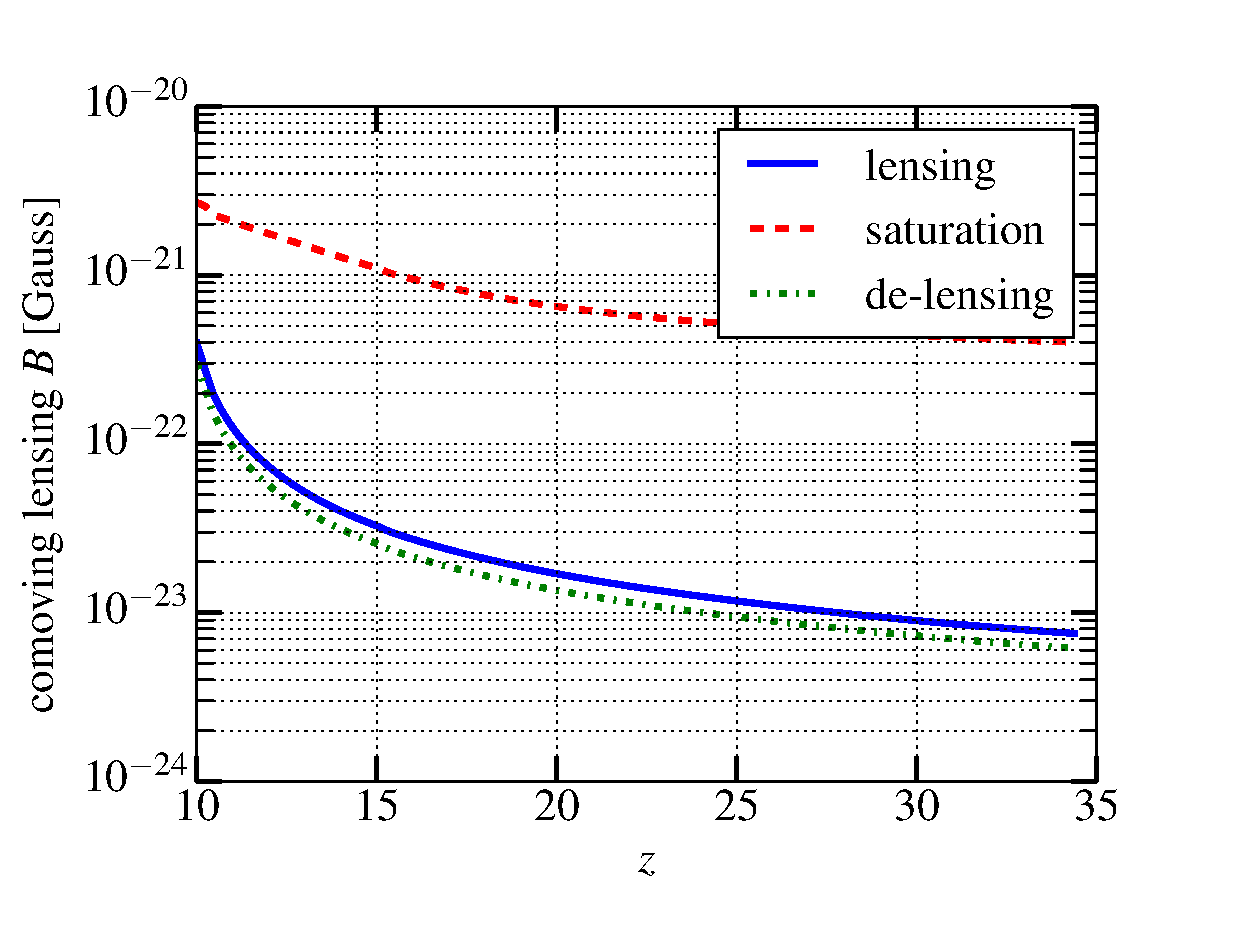
\includegraphics[scale=0.35]{delensingB.eps}
\caption{The $1\sigma$ comoving lensing magnetic field before and after de-lensing, as produced by the transverse shearing effect of weak lensing, compared to the saturation limit of our method.}
\label{fig:ps_B}
\end{figure}
\end{document}
